\chapter{Funktionen und ihre Graphen}
\section{Strecken, Verschieben und Spiegeln von Graphen}
\textit{Beispiel: Die Veränderung eines Graphen beschreiben}

$f(x) = -(x + 1)^4 + 2$ \\
$g(x) = x^4$ ($g$ hat einen Tiefpunkt $T$ bei $T(0|0)$

Der Graph von $f$ entsteht aus dem Graphen von $g$ durch Spiegelung an der $x$-Achse, Verschiebung um 1 LE\footnote{LE = Längeneinheit, FE = Flächeneinheit, VE = Volumeneinheit} in negative $x$-Richtung und Verschiebung um 2 LE in positive $y$-Richtung.\\
(Der Extrempunkt von $f$ lässt sich somit konstruieren: $H(-1 | 2)$)

\begin{definition}
    Symmetriekriterien: \\
    $f(x) = f(-x) \Longrightarrow \text{Achsensymmetrie zur $y$-Achse}$ \\ 
   $ f(-x) = -f(x) \Longrightarrow \text{Achsensymmetrie zum Ursprung}$ 
\end{definition}

\textit{Beispiel: Symetrie nachweisen}

\begin{minipage}{0.5\textwidth}
    (1) $f(x) = \sqrt{x^2 + 4}$ \\
    $f(-x) = \sqrt{(-x)^2 +4} = \sqrt{x^2 + 4} = f(x)$ \\ $G_f$ ist achsensymmetrisch zur $y$-Achse
\end{minipage}
\begin{minipage}{0.5\textwidth}
    (2) $f(x) = x \cdot e^{-x^2}$ \\
    $f(-x) = (-x) \cdot e^{-(-x)^2} = -x \cdot e^{-x^2} = -f(x)$ \\ $G_f$ ist punktsymmetrisch zum Ursprung
\end{minipage}

\section{Linearfaktordarstellung - mehrfache Nulstellen}

Aufschreib eigenständig - nachtragen!!

\section{Lösen von Gleichungen}

\textit{Beispiele}\\
(1) Zum lösen von Wurzelgleichungen wird immer folgendes Schema angewendet: \\ \textbf{Wurzelterm isolieren und dann Wurzel auflösen}
\begin{align*}
    \sqrt{x + 1} +1 &= 0 \\
    \sqrt{x + 1} & = -1 \\
    x + 1 &= 1 \\
    x &= 0 
\end{align*}

\textbf{Achtung!} Bei Wurzelgleichungen ist eine Probe nachher \textbf{immer} obligatorisch, da das quadrieren einer Wurzel keine Äquivalenzumformung ist.

\textbf{ENTWEDER: }

\textit{Probe:}\\
$\sqrt{0 + 1} + 1 = 2 \neq 0$ \\
Damit: $\mathbb{L} = \{\}$

\textbf{ODER:}

$\sqrt{x + 1} \neq -1 \ \forall x \in \mathbb{R}$ \\
Damit: $\mathbb{L} = \{\}$

(2) Bruchgleichungen lassen sich meist durch einfaches umformen lösen.
\begin{align*}
    \frac{x}{x - 1} &= \frac{3}{4} \qquad  \qquad |\cdot (x - 1); \ \cdot 4  \\
    4x &= 3x - 3 \\
    x &= -3
\end{align*}
Damit: $\mathbb{L} = \{-3\}$

\newpage 

(3) Bei Betragsgleichungen ist immer eine Fallunterscheidung und eine Probe notwendig. Es ist notwendig, bei einem beliebigem Fall, den Fall der Gleichheit einzuschließen. 
\begin{align*}
    |x - 4| &= 2x - 11 \\
\end{align*}
\begin{minipage}[t]{0.5\textwidth}
    1. Fall: $|x - 4| \geq 0$
    \begin{align*}
        x - 4 &= 3x - 11 \\
        x_1 &= 7
    \end{align*}
    \textit{Probe:} \\
    für $x_1 = 7$ gilt: 
    \begin{align*}
        |7 - 4| &= 2 \cdot 7 - 11 \\
        3 &= 3
    \end{align*}
\end{minipage}
\begin{minipage}[t]{0.5\textwidth}
    2. Fall: $|x - 4| < 0$
    \begin{align*}
        -(x - 4) &= 2x - 11 \\
        -x + 4 &= 2x - 11 \\
        x_2 &= 5
    \end{align*}
    \textit{Probe:}\\
    für $x_2 = 5$ gilt:
    \begin{align*}
        |5 - 4| &= 2 \cdot 5 - 11 \\
        1 &\neq -1
    \end{align*}
\end{minipage}

Damit: $\mathbb{L} = \{7\}$

\section{Trigonometrische Funktionen}

\begin{minipage}{0.55\textwidth}
    \begin{definition}
    Die Sinusfunktion $f$ mit $$f(x) = a \cdot \sin(b \cdot x) \text{ mit } a \neq 0 \text{ und } b > 0$$ hat die Amplitude $|a|$ und die Periode $p = \frac{2\pi}{b}$. \\
\end{definition}
\end{minipage}
\begin{minipage}{0.45\textwidth}
    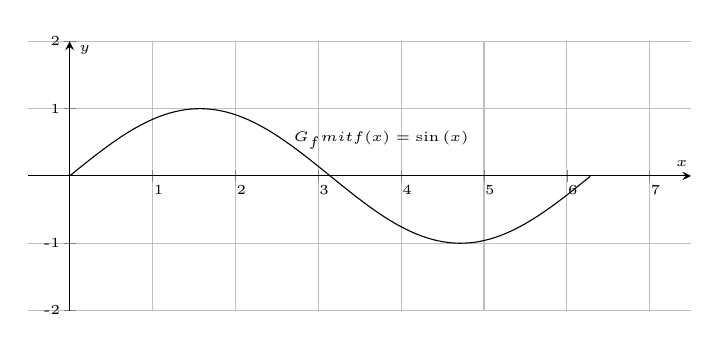
\begin{tikzpicture}[scale=1]
        \begin{axis}[clip=true, 
            ymin=-2, ymax=2, xmin=-.5, xmax=7.5,
            axis lines = middle, 
            xlabel=$x$, ylabel=$y$,
            xlabel style = {font=\tiny,xshift=0.5ex},
            ylabel style = {font=\tiny,yshift=0.5ex},
            ytick={-2,-1,...,1,2}, yticklabels={-2,-1,...,1,2}, ticklabel style = {font=\tiny,xshift=0.5ex},
            xticklabel style = {font=\tiny,yshift=0.5ex},
            xtick={1,2,...,6,7}, xticklabels={1,2,...,6,7}, grid = major, width= 10cm, height = 5cm]
        \addplot[samples= 100, domain=0:6.282]{sin(57.25*x)} node[right, pos=0.4]{\tiny$G_f \text{ mit } f(x) = \sin{(x)}$};
        \end{axis}
    \end{tikzpicture}
\end{minipage}
\begin{definition}
     Der Graph der Sinusfunktion $f$ mit $$f(x) = a \cdot \sin(b(x - c)) + d$$ ist zusätzlich um $c$ LE in positive $x$-Richtung und um $d$ LE in positive $y$-Richtung verschoben. \\ analoge Betrachtung: $f(x) = \cos(x)$
\end{definition}
